%% EXERCICIOS PARA INCLUÍR DENTRO DO CADERNO DE EXERCICIOS %%
%
% EXERCICIO.- ANÁLISE DA SECUENCIA: Dies irae
%
\section{Análise e comentario do gradual <<Viderunt omnes>>} \label{subsec:Viderunt-omnes}
%
\noindent
Analiza e realiza un breve comentario sobre a obra proposta. Lembra que para realizar a análise con partitura debemos seguir os pasos xa indicados na analise de audición do <<Puer natus est>> (ver o punto \ref{sec:Puer-natus} da páxina \pageref{sec:Puer-natus}). Unha vez obtidos e anotados os datos, realizamos o comentario. \\
Procura información sobre a mesma e realiza unha breve contextualización histórica, social e cultural tendo en conta a época ou período, forma (\ldots). Cita, xunto coa contextualización ao final do comentario, as fontes consultadas.\par
\subsection*{Puntos a indicar}
Debes indicar como mínimo na obra: modo, ámbito, estilo de canto, estrutura formal, clasificación no repertorio e contexto de interpretación


\vspace*{0.15cm}
%
%
% ----------------------
% Partitura de audición:
% ----------------------
\begin{figure}[h]
    \centering
    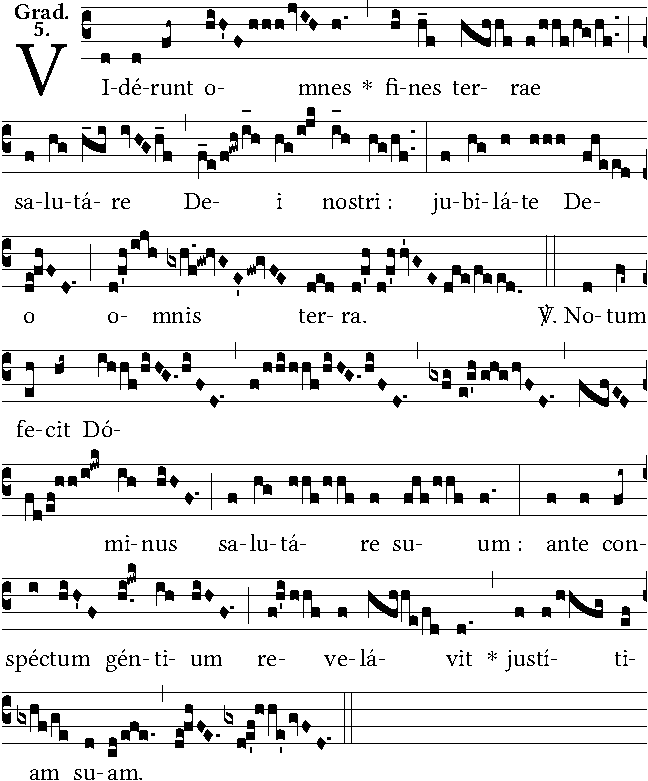
\includegraphics[width=0.70\textwidth]{audicions/viderunt-omnes.pdf}
    \caption{Gradual <<Viderunt omnes>>}
    \label{fig:Viderunt-omnes}
\end{figure}
% -----------------------

% RESUMO DA AUDICIÓN DO EXERCICIO
%
\vspace*{0.5cm}
\begin{ejercicio}[Comentario da audición: <<Viderunt omnes>>]
%\small{
%Redacta un breve comentario da obra. Ten en conta a análise feita:
%}

% ESPACIO PARA REDACTAR O COMENTARIO DA AUDICIÓN
%
%\small{Trátase dunha forma vocal menor, de estrutura ternaria; segundo o ámbito e estilo, obedece a un canto antifonal do propio da misa cantado a capella por un coro de voces masculinas; a textura monódica horizontal é propia do canto chá (Gregoriano) en estilo neumático na primeira sección e silábico na segunda, de ámbito reducido escrita no modo \textit{tetrardus auténtico} (VII)     }

        \vspace*{20.78cm}
\end{ejercicio}

